\documentclass{article}
\usepackage[utf8]{inputenc}
\usepackage{hyperref}
\usepackage[letterpaper, portrait, margin=1in]{geometry}
\usepackage{enumitem}
\usepackage{amsmath}
\usepackage{booktabs}
\usepackage{graphicx}

\usepackage{titlesec}

\titleformat{\section}
{\normalfont\Large\bfseries}{\thesection}{1em}{}[{\titlerule[0.8pt]}]
  
\title{Homework 7}
\author{Economics 7103}
  
\begin{document}
  
\maketitle

\section{Python}
\noindent 1. If I understood correctly, this policy is directed towards manufacturers. Since we have data on car sales in 2017, I believe it most likely includes already assembled cars that were made before the policy came into force. That's why I think there will still be cars longer than 225 inches that do not have specific safety technology. Additionally, it takes time to readjust to such manufacturing requirements, and governments usually provide some transition time before the policy is fully implemented. So, I expect more fuzzy R\&D.


\noindent 2.

\begin{figure}[h!]
    \centering
    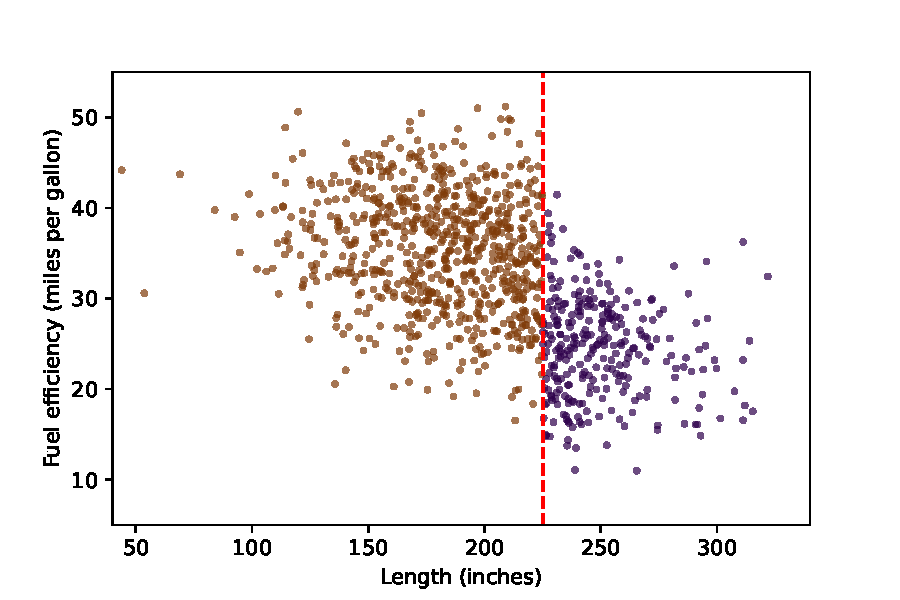
\includegraphics{homework 7/output/figure/scatterplot1.pdf}
    \caption{Scatter plot of Fuel efficiency in miles per gallon \& length}
    \label{fig:scatterplot1}
\end{figure}[h!]

\clearpage


title catter plot of vehicle fuel efficiency vs length
\noindent 3. 

\section{Stata}

\noindent 1.
\noindent 2. 

\end{document}